\documentclass[12pt,a4paper]{book}
\usepackage[utf8]{inputenc}
\usepackage[T1]{fontenc}
\usepackage[english]{babel}
\usepackage{amsmath}
\usepackage{amsfonts}
\usepackage{amssymb}
\usepackage{mathptmx}
\usepackage{mathpazo}
\usepackage{aligned-overset}
\usepackage{mathrsfs}
\usepackage{makeidx}
\usepackage{graphicx}
\usepackage{booktabs}
\usepackage{lscape}
\usepackage{tabularx}
\usepackage{times}%left=1.4cm, top=.8cm, right=1.4cm, bottom=1.8cm, footskip=.5cm
\usepackage[left=1.4cm, top=.8cm, right=1.4cm, bottom=1.8cm]{geometry}
\usepackage[section]{placeins}
\newtheorem{theorem}{Theorem}[section]
\newtheorem{dfn}{Definition}[section]
\newtheorem{note}{Note}[section]
\usepackage{titlesec}
\usepackage[style = apa, backend = biber, natbib = true]{biblatex}
\addbibresource{references.bib}
\usepackage{fancyhdr}
\pagestyle{fancy} % Turn on the style
\fancyhf{} % Start with clearing everything in the header and footer
% Set the right side of the footer to be the page number
\fancyfoot[R]{\thepage}

% Redefine plain style, which is used for titlepage and chapter beginnings
% From https://tex.stackexchange.com/a/30230/828
\fancypagestyle{plain}{%
	\renewcommand{\headrulewidth}{0pt}%
	\fancyhf{}%
	\fancyfoot[R]{\thepage}%
}
\usepackage{xcolor}
\makeatletter
%\renewcommand{\@makechapterhead}[]{%
	%	\vspace*{20 pt}%
	%	{\setlength{\parindent}{0pt} \raggedright\centring\bf \bfseries\normalfont{\thechapter\ #1\par\nobreak\vspace{20 pt}}}}
\makeatother
\titleformat{\section}{\bfseries\normalfont\centering\bf}{\thesection}{0em}{}
\begin{document}
	\pagestyle{plain}
	\openup 1 em
	\begin{titlepage}
		\pagenumbering{roman}
		%\addcontentsline{toc}{section}{Title Page}
		\begin{center}
			
			\begin{figure}[h]
				\begin{center}
					\includegraphics[width=0.30\linewidth, height=.20\textheight]{images/logo2}
				\end{center}
			\end{figure}
			
			{\normalfont{\textbf{UNIVERSITY OF ENERGY AND NATURAL RESOURCES, SUNYANI}}}\\
			\vspace{1.7cm}
			{\normalfont \textbf{THE VARIABILITY CLIMATE CHANGE IS RESPONSIBLE FOR IN VEGETATION LOSS IN GHANA}}
			
			
			\vspace{2.7cm}
			
			{\normalfont {\textbf{KALONG BONIFACE}}}\\
			{\normalfont {\textbf{FUGAH SELETEY MITCHELL}}}
			\vspace{1.7cm}
			
			
			\begin{center}
				{\normalfont \textbf{DEPARTMENT OF MATHEMATICS AND STATISTIC}\\
					\textbf{SCHOOL OF SCIENCE}}\\
				\vspace{5.3cm}
				
				
				{\normalfont \textbf{JUNE 2019}}
			\end{center}
			
		\end{center}
		
		\vfill
	\end{titlepage}
	\pagenumbering{roman}
	\begin{titlepage}
		\begin{center}
			{\normalfont \textbf{THE VARIABILITY CLIMATE CHANGE IS RESPONSIBLE FOR IN VEGETATION LOSS IN GHANA}}
			
			\vspace{3.7cm}
			{\normalfont {by}}\\
			\vspace{1cm}
			{\normalfont {Name - exams number\\ B.Sc. (Program) Location}}
			\vspace{1.7cm}
			
			
			\begin{center}
				{\normalfont A Thesis submitted to the Department of Mathematics and Statistics, School of Science, University of Energy and Natural Resources, Sunyani in partial fulfillment of the requirements for the degree of Bachelor of Science in Mathematics }\\
				\vspace{2cm}	
				{\normalfont JUNE 2019}
			\end{center}
			
		\end{center}
		
		\vfill
	\end{titlepage}	
	\newpage
	{\section*{DECLARATION AND CERTIFICATION}}
	\addcontentsline{toc}{section}{CERTIFICATION}
	Certified that the thesis entitled “\textbf{THE VARIABILITY CLIMATE CHANGE IS RESPONSIBLE FOR IN VEGETATION LOSS IN GHANA}”, submitted by
	{\normalfont {\textbf{Kalong Boniface}}} and {\normalfont {\textbf{Fugah Seletey Mitchell}}} to the \textbf{DEPARTMENT} , for the award of the degree of Doctor of Philosophy has been accepted by the external examiners and that the student has successfully defended the thesis in the viva voce examination held today.
	\\
	Candidate's Signature:	................................. \hspace\fill 
	Date: .................................	 \\
	\begin{center}\textbf{\normalfont \textbf{Supervisor's Certification}}\end{center}
	This study was carried out under the supervisory committee of (Names of all Supervisors) in accordance with the guidelines on supervisions of graduate studies.\\\\
	Major Supervisor's Name and Qualifications \\
	\\
	Signature:	................................. \hspace\fill 
	Date: .................................	 \\
	\begin{center}\textbf{\normalfont \textbf{Co-Supervisor's Certification}}\end{center}
	Co-Supervisor's Name and Qualifications\\
	\\
	Signature:	................................. \hspace\fill 
	Date: .................................	 \\
	\newline\\
	Co-Supervisor's Name and Qualifications\\
	\\
	Signature:	................................. \hspace\fill 
	Date: .................................	 \\
	
	
	\newpage
	\section*{\textbf{ABSTRACT}}
	\addcontentsline{toc}{section}{ABSTRACT}
	All thing change, but how we respond to change is our responsibility, to fare it or embrasse it. Resisting change leads to one fiat. Our own extinction. Time is a smybole of freedom and peace
	\newpage	
	\begin{center}\section*{DEDICATION}\end{center}
	\addcontentsline{toc}{section}{DEDICATION}
	
	Write dedication here   
	\newpage	
	\begin{center}\section*{ACKNOWLEDGMENTS}\end{center}
	\addcontentsline{toc}{section}{ACKNOWLEDGMENTS}
	
	Write Acknowledgment here
	
	\newpage
	\tableofcontents
	\addcontentsline{toc}{section}{TABLE OF CONTENTS}
	\newpage
	\listoftables
	\addcontentsline{toc}{section}{LIST OF TABLES}
	\newpage
	\listoffigures
	\addcontentsline{toc}{section}{LIST OF FIGURES}
	
	%	\renewcommand{\@makechapter}[]{%
		%	\vspace*{20 pt}%
		%	{\setlength{\parindent}{0pt} \raggedright \centering \bf \bfseries\normalfont{\thechapter \#1\par\nobreak\vspace{20 pt}}}}
	%\pagebreak
	\makeatother
	\titleformat{\chapter}{\bfseries\centering\normalfont\bf}{}{1em}{}
	\titleformat{\section}{\bfseries\normalfont\bf}{\thesection}{1em}{}
	
	\newpage
	\pagenumbering{arabic}
	\begin{flushleft}
		% Chapter 1

\chapter{CHAPTER ONE\\1.0 INTRODUCTION} % Main chapter title
\section{Introduction}
\label{Chapter1} % For referencing the chapter elsewhere, use \ref{Chapter1} 

%-------------------------------------------------------------------------------------

One would anticipate that the majority of emerging nations, which are still in the early stages of economic development and growth, would have a high forest cover and little deforestation. This, however, has not been the case. Ghana is a lower-middle-income nation that is still working toward middle-income classification. However, it has already begun to see a deforestation rate that is comparable to that of middle-income countries. The rapid population expansion, clearing of field for Galamsey operation,increased domestic need of wood for things like fuel, furniture, construction, and timber exports have all contributed to this trend, Bush fires in the 1980s, climate change, and lax law enforcement have all had an impact.

The purpose of this paper is to establish an understanding in time series analysis on remotely sensed data. Which will introduced us to the fundamentals of time series modeling, including decomposition, autocorrelation and modeling historical changes in Galamsey Operation in Ghana, the Cause,Dangers and it's Environmental impact.

Galamsey also known as "gather them and sell",\parencite{Owusu-Nimo2018} is the term given by local Ghanaian for illegal small-scale gold mining in Ghana . The major cause of Galamsey is unemployment among the youth in Ghana \parencite{Gracia2018}. Young university graduates rarely find work and when they do it hardly sustains them. The result is that these youth go the extra mile to earn a living for themselves and their family.

Another factor is that lack of job security. On November 13, 2009 a collapse occurred in an illegal, privately owned mine in Dompoase, in the Ashanti Region of Ghana. At least 18 workers were killed, including 13 women, who worked as porters for the miners. Officials described the disaster as the worst mine collapse in Ghanaian history \parencite{womendi2009}.

Illegal mining causes damage to the land and water supply \parencite{Ansah2017} . In March 2017, the Minister of Lands and Natural Resources, Mr. John Peter Amewu, gave the Galamsey operators/illegal miners a three-week ultimatum to stop their activities or be prepared to face the law \parencite{Allotey2017} . The activities by Galamseyers have depleted Ghana's forest cover and they have caused water pollution, due to the crude and unregulated nature of the mining process \parencite{gyekye}.

Under current Ghanaian constitution, it is illegal to operate as galamseyer.That is to dig on land granted to mining companies as concessions or licenses and any other land in search for gold. In some cases, Galamseyers are the first to discover and work extensive gold deposits before mining companies find out and take over. Galamseyers are the main indicator of the presence of gold in free metallic dust form or they process oxide or sulfide gold ore using liquid mercury.

Between 20,000 to 50,000, including thousands from China are believed to be engaged in Galamsey in Ghana.But according to the Information Minister 200,000 and nearly 3 million people, recently are now into Galamsey operation and rely on it for their livelihoods \parencite{goldgu2017}. Their operations are mostly in the southern part of Ghana where it is believe to have substantial reserves of gold deposits, usually within the area of large mining companies \parencite{Barenblitt2021} . As a group, they are economically disadvantaged. Galamsey settlements are usually poorer than neighboring agricultural villages. They have high rates of accidents and are exposed to mercury poisoning from their crude processing methods. Many women are among the workers, acting mostly as porters for the miners.

\section{Background of The Study}

As Galamsey is considered an illegal activity, they operations are hidden to the eyes of the authorities.So locating them is quite tricky ,but with satellite imagery ,it now possible to locate their operating and put an end to it. One of the features of Google Earth Engine is the ability to access years of satellite imagery without needing to download, organize, store and process this information. For instance, within the Satellite image

collection, now it possible to access imagery back to the 90's, allowing us to look at areas of interest on the map to visualize and quantify how much things has changed over time. With Earth Engine, Google maintains the data and offers it's computing power for processing.Users can now access hundreds of time series images and analyze changes across decades using GIS and R or other programming language to analyze these datasets.

\section{Problem Statement}

The Footprint of Galamsey is Spreading at a very faster rate, causing vegetation loss.Other factors accounting to vegetation loss may largely include climate change,urban and exurban development, bush fires. But not much works or research has been done to tell the extent to which Galamsey causes vegetation loss. This research attempts to segregate the variability climate is responsible for in vegetation loss so as to attribute the residual variability to Galamsey and other related activities such as bush-fires etc.

\section{Research Questions}

To address the challenge of the vegetation variability in this work, the following several statements were formed:

\begin{itemize}
	\item  Are there any changes in vegetation cause by Galamsey and Climate change in Ghana?
	
	\item Is there any relationship between vegetation and land surface temperature in Ghana?
\end{itemize}

\section{Research Objectives}

The purpose is to establish an understanding in time series analysis on remotely sensed data. We will be introduced to the fundamentals of time series modeling, including decomposition, auto-correlation and modeling historical changes.

\begin{itemize}
	\item Perform time series analysis on satellite derived vegetation indices
	
	\item Estimate the extent to which Galamsey causes vegetation loss in Ghana.
	
	\item Dissociate or single out the variability climate is responsible for in vegetation loss
\end{itemize}

\section{Significance Of The Study}

There have been significant changes in vegetation cover in Ghana over the past 30 years, and these dynamics are related strongly to climatic factors such as temperature and other factors. In this study, we want to examine the effects of climatic change on Ghana's vegetation during these thirty years.

This study allows us to explore climatic differences and climate-related drivers. Additionally, it offers a chance to research how climatic variability affects the ecosystem and human health. By merging climate and vegetation variation utilizing NDVI and EVI data to understand the relationship between vegetation and climate change under tropical climate conditions, it closes research gaps in Ghana. This study explores historical and projected vegetation and climate data, by sector, impacts, key vulnerabilities and what adaptation measures can be taken. It also explores the overview for a general context of how climate change is affecting Ghana.

\section{Limitation Of The Study}

The goal of time series modeling is to employ the simplest model feasible to account for as much data as possible while still developing an explanatory model of the data that does not over-fit the issue set.

Remote sensing data has additional limits that make this more difficult when dividing time series data into component pieces. It is almost certain that data from distant sensing will not provide the same level of precision.

Additionally, atmospheric factors can distort the visual findings, causing the vegetation's color to shift dramatically from image to image as a result of atmospheric factors (fog, ground moisture, cloud cover)%including chapters as standalone files
		% Chapter 2

\chapter{CHAPTER TWO\\2.0 LITERATURE REVIEW} % Main chapter title

\label{Chapter2} % For referencing the chapter elsewhere, use \ref{Chapter1} 

%----------------------------------------------------------------------------------------

% Define some commands to keep the formatting separated from the content 
%\newcommand{\keyword}[1]{\textbf{#1}}
%\newcommand{\tabhead}[1]{\textbf{#1}}
%\newcommand{\code}[1]{\texttt{#1}}
%\newcommand{\file}[1]{\texttt{\bfseries#1}}
%\newcommand{\option}[1]{\texttt{\itshape#1}}

%----------------------------------------------------------------------------------------
\section{Introduction}
Peralta \textit{et al.,} formulate a susceptible-vaccinated-infected-recovered (SVIR) model by incorporating the vaccination of newborns, vaccine age, and mortality induced by the disease into the SIR epidemic model. It is assumed that the period of immunity induced by vaccines varies depending on the vaccine-age. They performed a nonlinear stability analysis, by means of the Lyapunov function techniques and LaSalle's Invariance Principle for semiflows. They showed that the classical threshold condition for the effective reproductive number, $ R_{v} $, holds: $ R_{v} > 1 $; then the endemic steady $ E^{*} $ is globally asymptotically stable, whereas if $ R_{v} \leq 1$, then the infection-free steady state $ E_{0} $ is globally asymptotically stable. \parencite{peralta2015global}.

%---------------------------------------------------------------------------------------- 
		% Chapter 3

\chapter{CHAPTER THREE\\3.0 METHODOLOGY} % Main chapter title

\label{Chapter3} % For referencing the chapter elsewhere, use \ref{Chapter1} 

%-----------------------------------------------------------------------------------

\section{Introduction}
The techniques used to study our model are outlined in this chapter, together with a comprehensive explanation of the mathematical tools and constructs, theorems, lemmas, and their justifications.  The planning and execution processes of our technique make use of the R programming language. During the planning process, we considered where to get our data from and the procedures needed to build a time series model from the satellite data. We categorize our research as taking a quantitative approach. This research is specifically a causal-comparative experimental study with the goal of identifying the variability climate is responsible for in vegetation loss in Ghana.
 \section{Study Area}
 The Republic of Ghana, a nation in West Africa, will serve as the location for the experimental plots for this study. It shares borders with the Ivory Coast in the west, Burkina Faso in the north, and Togo in the east. It borders the Gulf of Guinea and the Atlantic Ocean to the south. Ghana's total size is 238,535 km2 (92,099 sq mi), and it is made up of a variety of biomes, from tropical rainforests to coastal savannas. Ghana, which has a population of over 31 million, is the second-most populous nation in West Africa, behind Nigeria.Accra, the nation's capital and largest city, as well as Kumasi, Tamale, and Sekondi-Takoradi, are other important cities

\section{DATA }
Data gathering. The majority of the quantitative data came from the Ghana Meteorological Agency and the Health Service. Rainfall, the highest temperature, and relative humidity are some of the meteorological data that were measured from 2010 to 2015 on a mean monthly basis. Additionally, based on monthly incidences for the Kumasi Metropolitan Area from 2000 to 2022, the data for EVI were obtained.

\subsection{Data Description and Inspection}

Data from a time series is a set of observations made in a particular order over a period of time. There is a chance for correlation between observations because time series data points are gathered at close intervals. To help machine learning classifiers work with time series data, we provide several new tools. We first contend that local features or patterns in time series can be found and combined to address challenges involving time-series categorization. Then, a method to discover patterns that are helpful for classification is suggested. We combine these patterns to create computable categorization rules. In order to mask low-quality pixels, we will first collect data from Google Earth Engine in order to choose  EVI values and Climate Change data.

Instead of analyzing the imagery directly, we will summarize the mean  Climate values. This will shorten the analysis time while still providing an attractive and useful map. We will apply a smoothing strategy using an ARIMA function to fix the situation where some cells may not have  EVI for a particular month. Once NA values have been eliminated, the time series will be divided to eliminate seasonality before the normalized data is fitted using a linear model. We will go to classify our data on the map and map it after we have extracted the linear trend.

Here, we made sure that we checked our data set for missing values and discovered there were none. The dataset’s number of columns is shown in the table below,
which also details the counts and datatype of various features in our dataset. No values are missing when there is a count of 133990. Anything below that denotes
the existence of unreported values.


 \subsection{Time Series Forecasting Using Stochastic Models}
 The selection of a proper model is extremely important as it reflects the underlying structure of the series and this fitted model in turn is
 used for future forecasting. A time series model is said to be linear or non-linear depending on whether the current value of the series is a
 linear or non-linear function of past observations.
 
 In general models for time series data can have many forms and represent different stochastic processes. There are two widely used linear time
 series models in literature.
 
 \emph{Autoregressive (AR)} and \emph{Moving Average (MA)} models, combining these two, the Autoregressive Moving Average (ARMA) and
 \emph{Autoregressive Integrated Moving Average (ARIMA)} models have been proposed in many literature. The \emph{Autoregressive Fractionally
 	Integrated Moving Average (ARFIMA)} model generalizes ARMA and ARIMA models. For seasonal time series forecasting, a variation of ARIMA. The
 \emph{Seasonal Autoregressive Integrated Moving Average (SARIMA)}  model is used.
 
 ARIMA model and its different variations are based on the famous Box-Jenkins principle Hipel and McLeod \parencite{hipel1994} and so these are also broadly known as the Box-Jenkins models.
\textbf{Vector Autoregression Model}\\
Model of vector autoregression. In econometrics, the Sims' vector autoregression (VAR) model has been widely employed to analyze multivariate time series. It provides better forecasting abilities than a univariate time series model and is a logical extension of the univariate autoregressive model to dynamic multivariate time series. Additionally, it identifies how each endogenous variable responds over time to a shock in both its own value and in every other variable. This method also enables the researcher to follow the data. The VAR model of order $p$ Sims \parencite{sims1980macroeconomics} proposed has the following basic form:
\begin{equation}
	y_{t} = A_{1}y_{t-1} + A_{2}y_{t-2} +\cdot+A_{p}y_{t-p}+ CD_{t} + \mu 
\end{equation}
Where $ y_{t} = \left( y_{1t},y_{2t},...,y_{kt}\right)'$ is a vector of K observable endogenous variables. For the purposes of this study, yt = $(EVI_{t}, Temperature_{t}, Rain_{}, Precipitation_{t},Drought_{t},Evaporation_{t})'$ where EVI denotes the value of vegetation conditions  each month, Temperature for both TMax and TMin, Rain denotes the amount of precipitation (mm), and Drought denotes the relative drought (\%). All deterministic variables, including constants, linear trends, and seasonal dummy variables, are contained in $D_{t}$. An unobservable zero-mean white noise process in K dimensions, $\mu_{t}$ has a positive definite covariance matrix $E(\mu_{t},\mu_{t}^{'}) = \sum_{\mu}$. We  apply different limits on the parameter matrices $A_{i}$ and C, which are of an appropriate dimension.
Generalized least squares is used to estimate the model's parameters.

\textbf{Augmented Dickey Fuller Test.} For stationarity, the Augmented Dickey Fuller \textbf{(ADF)} test is a unit root test. The alternative hypothesis varies slightly depending on the equation used, whereas the null hypothesis for the ADF test is that there is a unit root. The time series is steady, which is the most straightforward alternate theory. In time series analysis, unit roots can lead to unexpected outcomes.
\begin{align}        \Delta y_t &=  \color{red}\gamma y_{t-1} + \underbrace{\sum_{i=2}^{p} \beta_i \Delta y_{t-i+1}}_\text{control for serial correlation} + \epsilon_t  \\ \rightarrow (\tau1&)\quad H_0 : \color{red} {\gamma = 0} \\\\       \Delta y_t &=  \color{red}{\gamma} y_{t-1}  + \underbrace{\color{blue}{a_0}}_\text{constant} + \sum_{i=2}^{p} \beta_i \Delta y_{t-i+1} + \epsilon_t   \\ \rightarrow (\phi1&)\quad H_0 : \color{red} {\gamma = 0} \quad\&\quad\color{blue}{a_0 = 0}  \\\ \rightarrow (\tau2&)\quad H_0 : \color{red} {\gamma = 0}  \\\       \Delta y_t &=  \color{red}{\gamma} y_{t-1}  + \color{blue}{a_0}  + \underbrace{\color{green}{a_2} t}_{trend} + \sum_{i=2}^{p} \beta_i \Delta y_{t-i+1}  + \epsilon_t \\ \rightarrow (\phi2&)\quad H_0 : \color{red} {\gamma = 0} \quad\&\quad \color{blue}{a_0 = 0} \quad\&\quad \color{green}{a_2 = 0} \\ \rightarrow (\phi3&)\quad H_0 : \color{red} {\gamma = 0} \quad\&\quad\color{blue}{a_0 = 0}  \\ \rightarrow (\tau3&)\quad H_0 : \color{red} {\gamma = 0}    
 \end{align}

\textbf{Optimal Lag Length Selection Criteria.} \textbf{OLS} is used to estimate each of the system's individual equations. One of the following Information Criteria is minimized to determine the best lag order that is choosing optimal lag  to reduce residual correlation
\begin{center}
		\begin{tabular}{ll}
			\multicolumn{1}{c}{}Criteria &  Formular \\ \midrule
			AIC (n)  & = log det $ \displaystyle\left(\sum _{\mu}(n)\right)+ \frac{2}{T}nK^{2}$\\
			HQ(n)    & = log det  $ \displaystyle\left(\sum _{\mu}(n)\right)+ \frac{2logT}{T}nK^{2}$\\
			SC(n)    & = log det  $ \displaystyle\left(\sum _{\mu}(n)\right)+ \frac{logT}{T}nK^{2}$\\
			FPE(n)   & =          $\displaystyle \left(\frac{T + n^{*}}{T - n^{*}}\right)$det $\displaystyle \left(\sum_{\mu}(n)\right)$\\ \bottomrule
		\end{tabular}
\end{center}
where $ \displaystyle \sum_{\mu} (n)$ is the estimated by $T^{-1}\sum_{t=1}^{T}$
\section{Structural Analysis}
There are frequently many coefficients to comprehend, despite the fact that VAR coefficients describe the projected impact of a variable. Examining the model's residuals, which represent unforeseen contemporaneous events, is typically more prevalent. The next subsections explain some of the typical methods used for structural analysis of VAR models in a manner that is comparatively nontechnical.
\subsection{Causality Analysis} Both the Granger-causality and instantaneous causality were investigated. For both tests, the vector of endogenous variables is divided into two subvectors,$y_{1t}$ and $y_{2t}$ with dimensions $K_{1}$ and $K_{2}$,ctively, so that $K = K_{1} + K_{2}$ The subvector $y_{1t}$ said to be Granger-causal for
$y_{2t}$ if the past of $y_{1t}$ significantly helps predicting the future of $y_{2t}$ a the past of $y_{1t}$ one \parencite{granger1969investigating}. For testing this property,
a model of the form
\begin{equation}
	\displaystyle
	\left[ \begin{array}{c} y_{1t} \\ y_{2t}  \end{array} \right] \mbox{=} \sum_{i=1}^{p}\left[\begin{array}{cc}
		\alpha_{11,i} & \alpha_{12,i} \\
		\alpha_{21,i} & \alpha_{22,i} 
	\end{array}\right]\left[\begin{array}{c}
		y_{1,t-i}\\
		y_{2,t-i}
	\end{array}\right] + CD_{t} + \left[ \begin{array}{c}
		\mu_{1t}\\
		\mu_{2t}
	\end{array}\right]
\end{equation}
Where, $y_{1t}$ is not considered as  Granger-causal for $y_{2t}$ if and only if $ \alpha_{21,i} = 0,$ i = 1,2,...p.
Therefore, this null hypothesis is tested that at least one of the $\alpha_{21,i}$, has a positive value. The constraints are tested using an F-test statistic with a distribution of $F(pK_{1}K_{2}, KT - n^{*})$. Here, $n^{*}$ is the entire number of system parameters, including those for the deterministic term \parencite{lutkepohl2005new}. To test Granger-cause from $y_{2t}$ to $y_{1t}$, the roles of $y_{1t}$ and $y_{2t}$ can be switched.In other words, Granger causality responds to the question of whether previous values of the variable x may help anticipate future values of the variable y.

Instantaneous causality is defined as having a nonzero correlation between $\mu_{1t}$ and $\mu_{2t}$. Consequently, the null hypothesis is tested against the alternative 
\begin{equation}
	H_{0}: E\left(\mu_{1t},\mu_{2t}^{'} \right)
\end{equation}
is checked for instantaneous causation versus the alternative of nonzero covariance between the two error vectors. This hypothesis is investigated using a Wald test statistic.
\textbf{Analysis of impulse responses}: Exogenous and deterministic variables are viewed as fixed in impulse response analysis and can thus be removed from the system. Now, $y_{t}$ stands for the adjusted endogenous variables. The process $y_{t}$ has a Wold moving average (MA) representation if it is stationary \textbf{(I(0))}, which is represented by 
\begin{equation}
	y_{t} = \varPhi_{0}\mu_{t} + \varPhi_{1}\mu_{t-1} + \varPhi_{2}\mu_{t-2} + \dots
\end{equation}
Where $\varPhi_{0} =I_{K}$ and the $\varPhi_{s}$ can be computed recursively as 
\begin{equation}
	\varPhi_{s} = \sum_{j=i}^{s}\varPhi_{s-j}A_{j}, \quad s = 1,2,\dots,
\end{equation}
With $\varPhi = I_{K}$ and $A_{j} = 0 $ for $j>p$. The coefficients of this
representation may be interpreted as reflecting the responses
to impulses hitting the system. The \emph{(i,j)th} element of the matrices $\varPhi_{s},$ regarded as a function of \emph{s}, trace out the expected
response of $y_{i,t+s}$ to a unit change in $y_{it}$ holding constant all
past values of $y_{t}$
\section{ Forecast Error Variance Decomposition}
Denoting the $(i,j)th$ element of the orthogonalized impulse response
coefcient matrix $\theta_{n}$ by $\theta_{ij,n}$, the variance of the forecast error $\left(y_{k,T+h}-y_{k,T+h|T}\right)$ is 
\begin{equation}
	\begin{split}
		\displaystyle
		\sigma^{2}_{k}(h) & = \sum^{h-1}_{n=0}\left(\theta^{2}_{k1,n} + \cdot+ \theta^{2}_{kK,n}\right) \\
		& =\sum^{K}_{j=1}\left(\theta^{2}_{kj,0} + \cdot+ \theta^{2}_{kj,h=1}\right)
	\end{split}
\end{equation}
The term $\displaystyle \left(\theta^{2}_{kj,0} + \cdot+ \theta^{2}_{kj,h=1}\right) $ is interpreted as the contribution
of variable \emph{j} to the \emph{h}-step forecast error variance of variable
\emph{k}.  Dividing the above terms by $\displaystyle \sigma^{2}_{k}(h)$ gives the percentage \emph{j} to the \emph{h}-step forecast error variance of variable
\emph{k}, 
\begin{equation}
	\omega_{kj}(h) =\frac{\left(\theta^{2}_{kj,0} + \cdot+ \theta^{2}_{kj,h=1}\right)}{\sigma^{2}_{k}(h)}
\end{equation}
\section{Forecast Performance Measures}

While applying a particular model to some real or simulated time series, first the raw data is divided into two parts (\textbf{Training Set and
	Test Set}). The observations in the training set are used for constructing the desired model. Often a small sub-part of the training
set is kept for validation purpose and is known as the \textbf{Validation Set}. Sometimes a preprocessing is done by normalizing the data or taking logarithmic or other transforms. One such famous technique is the Box-Cox Transformation {[}23{]}. Once a model is constructed, it is used for generating forecasts. The test set observations are kept for verifying how accurate the fitted model performed in forecasting these values. If necessary, an inverse transformation is applied on the forecast values to convert them in original scale. In order to judge the forecasting accuracy of a particular model or for evaluating and comparing different models, their relative performance on the test dataset is considered.

Due to the fundamental importance of time series forecasting in many practical situations, proper care should be taken while selecting a particular model. For this reason, various performance measures are proposed in literature to estimate forecast accuracy and to compare different models. These are also known as performance metrics {[}24{]}. Each of these measures is a function of the actual and forecast values of the time series.

% this line fixes the vertical padding of text inside the cells
\renewcommand{\arraystretch}{1.4}
%\begin{sidewaystable}
%	\caption{Description of Various Forecast Performance Measures}
%	\label{tab:my-table}
%	\resizebox{\columnwidth}{2.5cm}
%	\begin{tabularx}{\textwidth}{|L{2cm}|X|L{2cm}|L{2cm}|X|}{lllll}
%		\hline
%		& \multicolumn{4}{l}{\cellcolor[HTML]{C0C0C0}}{Error Matrix} \\ \midrule    
%		
%		& \multicolumn{1}{l}{MAE}
%		& \multicolumn{1}{l}{RMSE}
%		& \multicolumn{1}{l}{MSE}
%		& \multicolumn{1}{l}{MAPE} \\
%		\midrule
%		\multicolumn{13}{l}{}                                \\
%		\\\multicolumn{13}{l}{}   \\ 
%		
%		\multicolumn{13}{c}{Where: In each of the forthcoming definitions, $y_{t }$ is the actual value,$f_{t}$ is the forecast value, $e_{t} = y_{t} - f_{t}$ is the forecast error and n is the size of the test set. Also, $\displaystyle \bar{y} = \frac{1}{n}\sum_{t=1}^{n}y_{t}$ is the test mean and $\displaystyle \sigma^{2} = \frac{1}{n-1}\sum_{t=1}^{n}(y_{t}-\bar{y})^{2}$is the test variance.}                                \\\hline\hline
%		Formulas 
%		& $\displaystyle MAE = \frac{1}{n}\sum_{t=1}^{n}|e_{t}|$ \\
%		& $\displaystyle RMSE = \sqrt{MSE} = \sqrt {\frac{1}{n}\sum_{t=1}^{n}e^{2}_{t}}$ \\
%		& $\displaystyle MSE = \frac{1}{n}\sum_{t=1}^{n}e^{2}_{t}$\\
%		& $\displaystyle MAPE= \frac{1}{n}\sum^{n}\left(\frac{e_{t}}{y_{t}}\right)$ \\ \bottomrule
%		
%		\multicolumn{13}{l}{}                                \\
%	\end{tabularx}%
%	
%	
%\end{sidewaystable}
\newpage
\subsection{Description of Various Forecast Performance Measures}
\textbf{MAPE}\\
This measure represents the percentage of average absolute error occurred. It is independent of the scale of measurement, but affected by data transformation.It does not show the direction of error. MAPE does not penalize extreme deviations. In this measure, opposite signed errors do not offset each other.
\\
\textbf{MSE}\\
It is a measure of average squared deviation of forecast values. As here the opposite signed errors do not offset one another, MSE gives an overall idea of the error occurred during forecasting. It penalizes extreme errors occurred while forecasting. MSE emphasizes the fact that the total forecast error is in fact much   affected by large individual errors, i.e. large errors are much expensive than small errors. MSE does not provide any idea about the direction of overall error. MSE is sensitive to the change of scale and data transformations. Although MSE is a good measure of overall forecast error, but it is   not as intuitive and easily interpretable as the other measures discussed before. 

\textbf{RMSE}\\
RMSE is nothing but the square root of calculated MSE. All the properties of MSE hold for RMSE as well.

\textbf{MAD}\\
measures the average absolute deviation of forecast values from   original ones.It shows the magnitude of overall error, occurred due to forecasting.In MAE, the effects of positive and negative errors do not cancel out.Unlike MFE, MAE does not provide any idea about the direction of  errors. For a good forecast, the obtained MAE should be as small as possible. Like MFE, MAE also depends on the scale of measurement and data   transformations.Extreme forecast errors are not panelized by MAE.\\
%\begin{landscape}
	\begin{table}[]
		\begin{tabularx}{\textwidth}{@{}llll@{}}
			\toprule \hline
			MAE	&  RMSE   &  MSE   &  MAPE  \\ \midrule
			\hline
			$\displaystyle  \frac{1}{n}\sum_{t=1}^{n}|e_{t}|$	& $\displaystyle  \sqrt{MSE} = \sqrt {\frac{1}{n}\sum_{t=1}^{n}e^{2}_{t}}$    & $\displaystyle  \frac{1}{n}\sum_{t=1}^{n}e^{2}_{t}$    & $\displaystyle  \frac{1}{n}\sum^{n}\left(\frac{e_{t}}{y_{t}}\right)$   \\ \bottomrule
			
		\end{tabularx}
	\end{table}
%\end{landscape}
Where: In each of the forthcoming definitions, $y_{t }$ is the actual value,$f_{t}$ is the forecast value, $e_{t} = y_{t} - f_{t}$ is the forecast error and n is the size of the test set. Also, $\displaystyle \bar{y} = \frac{1}{n}\sum_{t=1}^{n}y_{t}$ is the test mean and $\displaystyle \sigma^{2} = \frac{1}{n-1}\sum_{t=1}^{n}(y_{t}-\bar{y})^{2}$is the test variance.


		% Chapter 3

\chapter{CHAPTER FOUR\\4.0 DATA ANALYSIS AND RESULTS} % Main chapter title
\section{Introduction}
In this chapter, we present the results of the data analysis. We also interpret and discuss the results. 

\subsection{Preliminary Results}
The study's data set includes time series of monthly EVI cases for the study area as well as various climatic factors like precipitation,evaporation, temperature (Tmin and Tmax), drought and drought . After extracting all the data from  Google Earth Engine, there was a chance for correlation between observations because time series data points are gathered at close intervals. Instead of analyzing the imagery directly, we  summarize the data through descriptive statistics for the six variables under consideration which are shown in Table \ref{table:Summary Statistics}. The numbers for EVI are 0.3945, 0.8672, and 0.7192, respectively, which are the minimum, maximum, and average levels. In terms of climatic factors, the minimum, maximum, and average values of Precipitation are 0.1203mm, 12.3576mm, and 3.9604mm, respectively. In contrast, the minimum, maximum, and average values of maximum temperature are 274.4C, 348.2C, and 309.3C, respectively. The original data's time series plots are shown in Figure \ref{fig:TimeSeries}, which clearly shows that both EVI and the climatic variables under consideration are seasonal. 
\subsection{Variable \& Parameter Definition}
Find in the tables ~\ref{label:Variable}  the definition of variables and parameters respectively as used in this study. 
\begin{table}
	\label{label:Variable}
	\caption{Variable Definition.}
	\centering
	\begin{tabularx}{\textwidth}{ll}
		\hline\noalign{\smallskip}
		Variable & Definition \\ 
		\noalign{\smallskip}\hline\noalign{\smallskip}
	     EVI          & Susceptible individuals \\  
		Precipitation & Exposed individuals \\ 
		Evaporation   & Actual evapotranspiration, derived using a one-dimensional soil water balance model\\ 
		TempMin       & Minimum Temperature \\ 
		TempMax       & Maximum Temperature \\
		Drought       &Palmer Drought Severity Index\\
		\hline\noalign{\smallskip}
	\end{tabularx}
\end{table}
\subsection{Selection of Variables}
The purpose of this part is to examine how we got our answer and variables. First, we extract all our climatic data using one of the coordinate in these cells . 
To shorten the analysis time while still providing an attractive and useful map. We apply a smoothing strategy using an ARIMA function to fix the situation where some cells do not have EVI for a particular month. Once NA values have been eliminated, the time series will be divided to eliminate seasonality before the normalized data is fitted using a linear model. We will go to classify our data on the map and map it after we have extracted the linear trend.

To help machine learning classifiers work with time series data, we provide several new tools. We first contend that local features or patterns in time series can be found and combined to address challenges involving time-series categorization. Then, a method to discover patterns that are helpful for classification is suggested. We combine these patterns to create computable categorization rules.
 
\textbf{Note} that the Analysis was divided into two, the uni-variate and Multivariate Analysis, where we use the uni-variate analysis to show the foot print of vegetation loss and multivariate to analysis how climatic variable are also contributing to such events.In that case we mask low-quality pixels, by  first collecting data from Google Earth Engine in order to choose  EVI values and Climate Change data. The Plot \ref{fig:TimeSeries}  shows the first difference in the data provides evidence of stationarity in EVI variables.Which we used to create the map. 
\begin{table}[]
	\label{DataFrame}
	\caption{Data Collected from 2000-2022 on Google Earth Engine }
	\centering
	\begin{tabularx}{\textwidth}{@{}cllllll@{}}
		\toprule
		& \multicolumn{1}{c}{Vegetation Indices}   & \multicolumn{3}{c}{Climate Change}  \\ \midrule
		\multicolumn{1}{c}{Date} & \multicolumn{1}{c}{EVI} & \multicolumn{1}{c}{Precipitation} & \multicolumn{1}{c}{Evaporation} & \multicolumn{1}{c}{TempMin} & \multicolumn{1}{c}{TempMax} &\multicolumn{1}{c}{Drought}\\ \midrule
		
		
		2000-01-01&	-0.38280560&	1.0344619&	2.936857e-05&	217.1814&	315.8379&	-86.12496\\
		2000-02-01&	-0.08346374&	0.9917288&	2.634354e-05&	210.7751&	325.4743&	-168.35120\\
		2000-03-01&	0.46029681&	3.2132809&	2.927312e-05&	232.6620&	332.0389&	-220.69199\\
		2000-04-01&	0.68380747&	5.1810527&	4.515878e-05&	224.0424&	321.6810&	-190.38286\\
		2000-05-01&	0.25644143&	6.7150908&	4.758059e-05&	228.8765&	318.3983&	-210.67141\\
		2000-06-01&	-0.28410451&	8.2797964&	4.928518e-05&	222.4945&	295.6937&	-209.06835\\\bottomrule
		
	\end{tabularx}
\end{table}
\begin{table}[]
	\label{table:Summary Statistics}
	\caption{Summary statistics for Climate Date and Vegetation Loss In Ghana}
	\centering
	\begin{tabularx}{\textwidth}{|l*{3}{X|}*{3}{X|}}
		\toprule
		                   & Min.      & 1st Qu. & median   & Mean     & 3rd Qu   & Max.  \\ \midrule
		EVI                &   0.3945  & 0.6423  & 0.7242   & 0.7168   & 0.8168   &0.8672 \\
		Precipitation      &   0.1203  & 2.0311  & 3.5497   &  3.9427  & 5.4892   &12.3576 \\
		Evaporation        & 1.682e-05 &3.595e-05&4.215e-05 &4.033e-05 & 4.560e-05&5.432e-05 \\
		TempMin            &   194.0   & 220.6   & 225.6    & 225.1    & 230.5    &242.7 \\
		TempMax            &   274.4   & 294.1   & 313.8    & 309.0    &  322.2   &348.2 \\ 
		Drought            &  -1354.42 & -339.45 & -228.47  &-257.12   & -89.24   &369.64 \\ \bottomrule
	\end{tabularx}
\end{table}
\begin{figure}
	\centering
	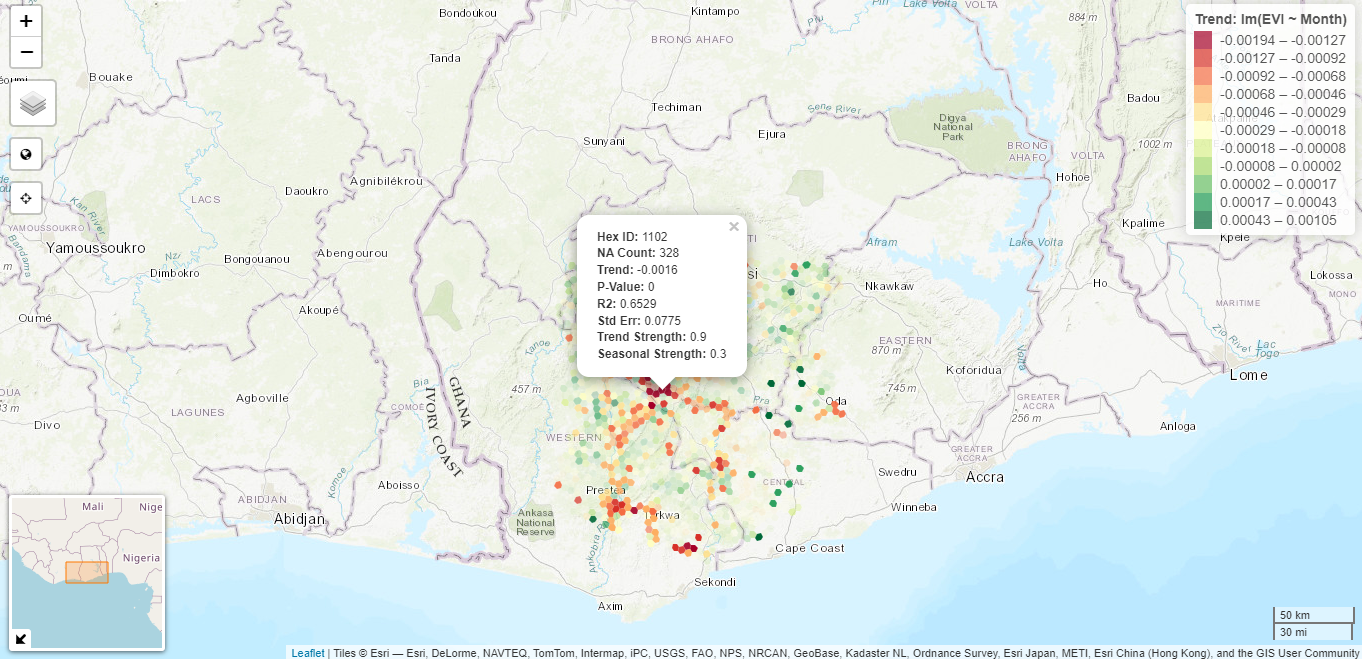
\includegraphics[width=0.9\linewidth]{images/Map}
	\caption{EVI Classification}
	\label{fig:map}
\end{figure}


For mulitvariate analysis, we checked for the Pearson’s correlation between our target variable’s and the covariates’ which are presented in the Figure \ref{fig:Correlation} below
\begin{figure}
	\centering
	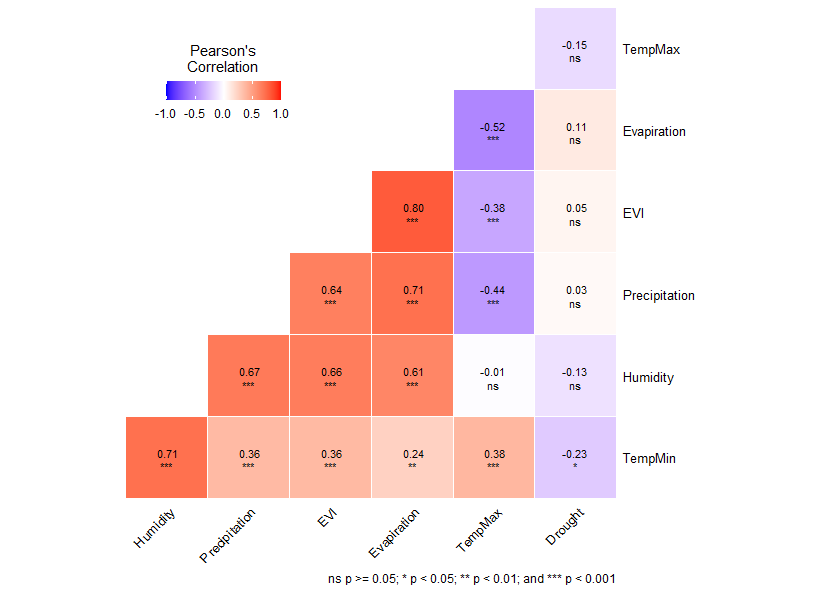
\includegraphics[width=0.9\linewidth]{images/Correlation}
	\caption{Pearson’s Correlation Between Variables}
	\label{fig:Correlation}
\end{figure}

\subsection{Multicollinearity}
Although we have known about our study's target variable, EVI, from the outset, picking the covariates was a challenge. The following variables, with the exception of EVI, were intended to be used as covariates until it was discovered that multicollinearity among the covariates increases the sum of squared error.We employed the Variance Inflation Factor (VIF) to test for multi-collinearity, and the findings is shown in Table\ref{table:VIF}

In order for our VIF score to fall between the ranges of 1 and 5, a piece of code was executed that automatically deleted variables with the highest VIF scores. We statistically concluded that the variables Drought, TempMin, Precipitation, TempMax, and Evaporation will explain our target variable.
\begin{center}
	\begin{table}
	\label{table:VIF}
	\caption{Best Variance Inflation Factor}
	\centering
	\begin{tabular}{|l|l|}
		\hline\hline
		Parameter	& Values \\
		\hline\hline
		Predictors	& 5 \\
		VIF	& 2.373 \\
		Condition number 	& 7.939\\
		Determinant 	& 0.2260766568 \\
		Selected 	& Drought, TempMin, Precipitation, TempMax, Evaporation \\
		Removed 	&  drought\\
		\hline
	\end{tabular}
  \end{table}
\end{center}

\subsection{Stationarity and Differencing}
Before building our models we first checked  if the series is stationary.We used the R program to do the ADF test, and we looked at many ADF test statistics to determine whether a unit root existed. This is essential to the VECM model and the VAR model in particular. That is, we needed to be determined that the time series is constant in mean and variance, and not dependent on time.Here, we look at a couple of methods for checking stationarity. If the time series is provided with seasonarity, a trend, or a change point in the mean or variance, then the influences need to be removed or accounted for. We use the Augmented Dickey–Fuller (ADF) t-statistic test to find if the series has a unit root (a series with a trend line will have a unit root and result in a large p-value)\parencite{dickey1979distribution}.The test, shown in Table \ref{table:(ADF) unit root test}, approved the unit root hypothesis for all time series taken into account, suggesting that the relationships between the numerous variables investigated below are not fictitious.
\label{Chapter4} % For referencing the chapter elsewhere, use \ref{Chapter1} 
\begin{table}[]
	\label{table:(ADF) unit root test}
	\caption{Augmented Dickey Fuller (ADF) unit root test }
	\centering
	\addtolength{\tabcolsep}{4pt}
	\begin{tabularx}{\textwidth}{@{}cllllll@{}}
		\toprule
		& \multicolumn{3}{c}{EVI}   & \multicolumn{3}{c}{Precipitation}  \\ \midrule
		\multicolumn{1}{c}{} & \multicolumn{1}{c}{tau3} & \multicolumn{1}{c}{phi2} & \multicolumn{1}{c}{phi3} & \multicolumn{1}{c}{tau3} & \multicolumn{1}{c}{phi2} &\multicolumn{1}{c}{phi3}\\ \midrule
		
		Test-Statistics&-12.23373&49.89733&74.84565&-12.90546&55.54404&83.31586\\
		1pct&-3.98&6.15&8.34&-3.98&6.15&8.34\\
		5pct&-3.42&4.71&6.30&-3.42&4.71&6.30\\
		10pct&-3.13&4.05&5.36&-3.13&4.05&5.36\\ \bottomrule
		& \multicolumn{3}{c}{TempMin}   & \multicolumn{3}{c}{TempMax}  \\ \midrule
		\multicolumn{1}{c}{} & \multicolumn{1}{c}{tau3} & \multicolumn{1}{c}{phi2} & \multicolumn{1}{c}{phi3} & \multicolumn{1}{c}{tau3} & \multicolumn{1}{c}{phi2} &\multicolumn{1}{c}{phi3}\\ \midrule
		
		Test-Statistics&-9.292711&28.810535&43.191412&-9.219737&28.363876&42.545576\\
		1pct&-3.98&6.15&8.34&-3.98&6.15&8.34\\
		5pct&-3.42&4.71&6.30&-3.42&4.71&6.30\\
		10pct&-3.13&4.05&5.36&-3.13&4.05&5.36\\ \bottomrule
		
		& \multicolumn{3}{c}{Evaporation}   & \multicolumn{3}{c}{Drought}  \\ \midrule
		\multicolumn{1}{c}{} & \multicolumn{1}{c}{tau3} & \multicolumn{1}{c}{phi2} & \multicolumn{1}{c}{phi3} & \multicolumn{1}{c}{tau3} & \multicolumn{1}{c}{phi2} &\multicolumn{1}{c}{phi3}\\ \midrule
		
		Test-Statistics&-11.37318&43.16267&64.74007&-3.421750&3.915871&5.862217\\
		1pct&-3.98&6.15&8.34&-3.98&6.15&8.34\\
		5pct&-3.42&4.71&6.30&-3.42&4.71&6.30\\
		10pct&-3.13&4.05&5.36&-3.13&4.05&5.36\\
		
		\midrule\bottomrule
	\end{tabularx}
\end{table}
\section{VAR Estimation} With 12 lags for each variable in each equation, a VAR model of the monthly EVI and Climate change variables was estimated. There are 4x12 unconstrained coefficients in each equation, plus one for a constant and one for a trend. Four tests were examine, the Final Prediction Error (FPE) test, the Hannan Quinne (HQ) test, the Information Criteria proposed by Akaike (AIC), and the Schwarz (SC) test were used to determine the appropriate number of lags. The results of all four tests suggested that up to 12 lagged monthly values would be sufficient. All the dynamics in the data are captured and employed in this analysis thanks to a lag duration of 12. (Table \ref{table:Optimal lag}).

\begin{table}[]
	\label{table:Optimal lag}
	\caption{Optimal lag length selection}
	\centering
	\addtolength{\tabcolsep}{25pt}
	\begin{tabularx}{\textwidth}{@{}lllll@{}}
		\toprule
	 Lag  &	AIC(n)&	HQ(n)&	SC(n)&	FPE(n)\\\midrule
	1&	-8.242332&	-8.006335&	-7.655762&	0.0002633\\
	2&	-9.304816&	-8.866535&	-8.215470&	0.0000910\\
	3&	-9.743066&	-9.102502&	-8.150946&	0.0000588\\
	4&	-10.142686&	-9.299839&	-8.047791&	0.0000395\\
	5&	-10.286777&	-9.241647&	-7.689107&	0.0000343\\
	6&	-10.338471&	-9.091058&	-7.238027&	0.0000328\\
	7&	-10.345081&	-8.895385&	-6.741861&	0.0000328\\
	8&	-10.344697&	-8.692718&	-6.238702&	0.0000331\\
	9&	-10.310857&	-8.456595&	-5.702089&	0.0000347\\
	10&	-10.251454&	-8.194908&	-5.139910&	0.0000374\\
	11&	-10.250272&	-7.991444&	-4.635954&	0.0000382\\
	12&	-10.295256&	-7.834144&	-4.178163&	0.0000374\\
		 \bottomrule
	\end{tabularx}
\end{table}
\begin{figure}
	\centering
	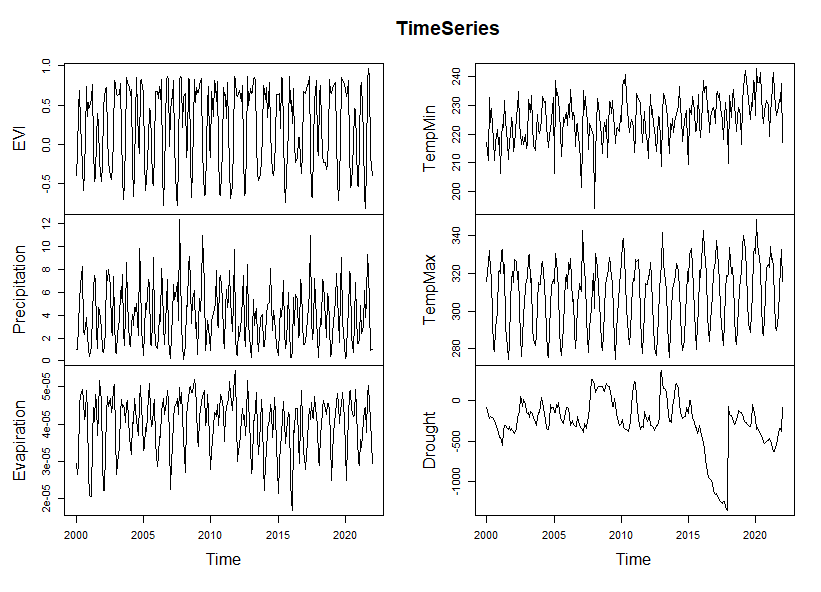
\includegraphics[width=0.9\linewidth]{images/TimeSeries}
	\caption{Time Series Plot of all Variables}
	\label{fig:TimeSeries}
\end{figure}
\begin{table}[]
	\label{table:Prediction}
	\caption{EVI forecast for the next 12 month.}
	\centering
	\addtolength{\tabcolsep}{25pt}
	\begin{tabularx}{\textwidth}{@{}lllll@{}}
		\toprule
   Month       & Forecast& Lower  &   Upper  &CI\\
   \bottomrule
Feb &-0.07548865& -0.65614302& 0.5051657& 0.5806544\\
Mar & 0.14803164& -0.56646127& 0.8625245& 0.7144929\\
Apr & 0.69105704& -0.04392727& 1.4260414& 0.7349843\\
May & 0.72499702& -0.05679272& 1.5067868& 0.7817897\\
Jun & 0.44066359& -0.41564183& 1.2969690& 0.8563054\\
Jul &-0.11537243& -0.98453117& 0.7537863& 0.8691587\\
Aug &-0.37165805& -1.24946226& 0.5061462& 0.8778042\\
Sep &-0.16672258& -1.05855108& 0.7251059& 0.8918285\\
Oct & 0.16015717& -0.73872579& 1.0590401& 0.8988830\\
Nov &  0.37177202& -0.53806829& 1.2816123& 0.9098403\\
% &  0.38160641& -0.53535068& 1.2985635& 0.9169571\\
% &  0.42144590& -0.49952777& 1.3424196& 0.9209737\\
		 \bottomrule
\end{tabularx}
\end{table}
\begin{table}[]
	\label{Optimal lag}
	\caption{Granger causality tests.}
	\centering
	
	\addtolength{\tabcolsep}{3pt}
	\begin{tabularx}{\textwidth}{@{}lllll@{}}
	\hline
	Cause variable &Null hypothesis& F-value& p-value& Decision\\
	\hline\hline
Precipitation	& does not Granger-cause EVI &2.1563  & 0.01464  & Reject the null hypothesis  \\
	\hline
Evaporation	& does not Granger-cause EVI & 1.5398 & 0.1112 &Fail to Reject the null hypothesis  \\
	\hline
TempMin	&  does not Granger-cause EVI&3.0049  & 0.0006276 &Reject the null hypothesis  \\
	\hline
TempMax	& does not Granger-cause EVI &2.7462  & 0.001685 &Reject the null hypothesis  \\
	\hline
Drought	& does not Granger-cause EVI & 0.9235 & 0.5241 &Fail to Reject the null hypothesis \\
	\hline
\end{tabularx}
\end{table}
\section{Impulse Response Analysis}
The dynamic interactions between EVI and the Climatic variables of the VAR (12) process were examined using impulse response analysis. Figure ~\ref{fig:impose} shows the orthogonal impulse response of EVI(Vegetation Condition) to the climate factors. The reaction of EVI exhibits a clear variation; the seventh month (July) has the largest negative effect of maximum temperature on EVI while we can see a rise in the Evaporation side and the third month has the lowest adverse effect (March). Additionally, the third month (March) is when drought has the most positive impact on EVI, whereas the tenth month (October) is when precipitation has the greatest good impact (October).
\begin{figure}
	\centering
	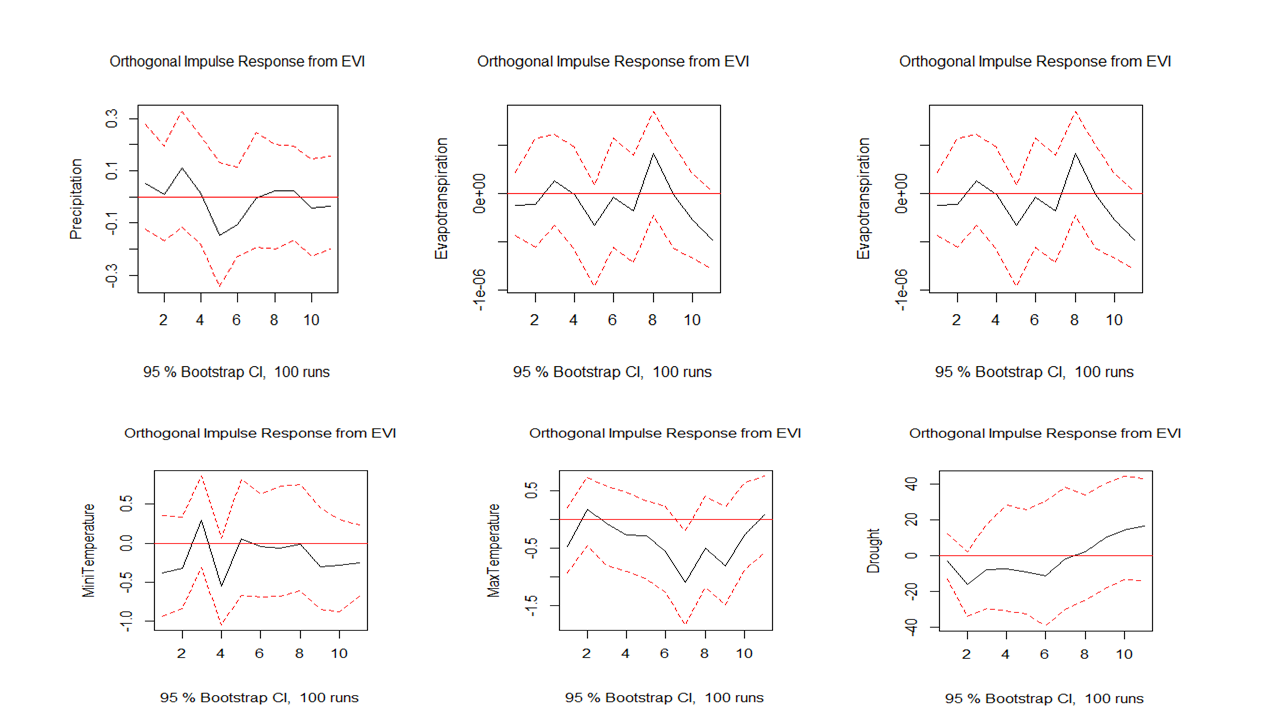
\includegraphics[width=1\linewidth]{images/impose}
	\caption{Impulse Response Analysis}
	\label{fig:impose}
\end{figure}
\subsection{ Decomposition of Variance}
In order to evaluate VAR models, many people use forecast error variance decomposition (FEVD). Figure ~\ref{fig:fevd} displays the results for the FEVD for EVI and the climate factors. The findings show that, on average, past values EVI(Vegetation Condition)  account for about 85.67\% of the variability in the trend of EVI, while past innovations in maximum temperature account for a sizable percentage (around 5.65\%) of the variability in the trend of EVI. Additionally, although earlier advances in Evaporation data have been able to account for around 3.10 percent of the variability in the trend of EVI, past innovations in relative Precipitation have only been able to account for 0.58 percent of that variability.
\begin{figure}
	\centering
	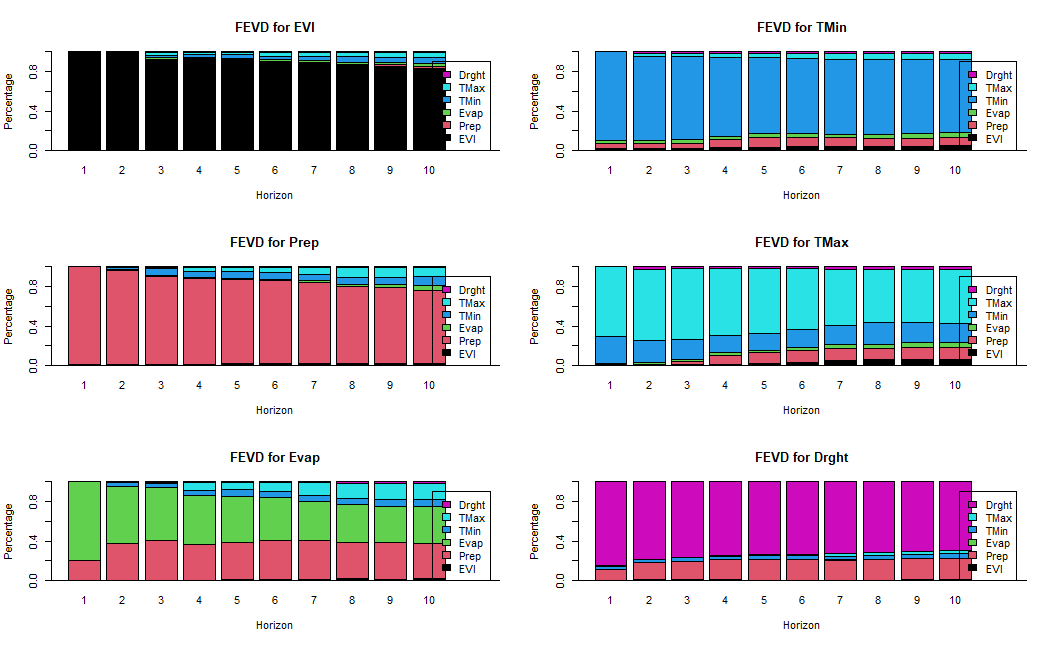
\includegraphics[width=0.9\linewidth]{images/fevd}
	\caption{Forecast Error Variance Decomposition (FEVD)}
	\label{fig:fevd}
\end{figure}
\subsection{Forecast for EVI} Future EVI  cases can be predicted using the created VAR (12) model as a predictive model. Figure  and Table  both revert the forecasts for the number of differed EVI during the first half of 2022 to the original level. These predictions \ref{table:Prediction}

\subsection{Prediction Accuracy} Regardless of whether the forecasting mistake is positive or negative, the mean absolute percentage error (MAE) gives a general idea of the average size of forecasting error represented as a \% of the actual observed number .In this case the closer MAE is to zero (0) the more  accurate the model is. The fitted model's MAE is calculated to be \textbf{2.065071e-01} using (10) which suggests that its projections may be quite accurate .~\ref{label: Accuracy}
	\begin{center}
		\begin{table}
			\label{label: Accuracy}
			\caption{Forecast Accuracy on EVI Training set}
			\centering
			\small
			\addtolength{\tabcolsep}{-4pt}
			\begin{tabular}{llllllll}
				\hline\hline
				& ME	       & RMSE        &MAE          &MPE   &MAPE& MASE        &ACF1 \\
				&-1.384005e-17& 2.665621e-01& 2.065071e-01&-Inf  &Inf & 0.00131& 0.0123\\
				\hline
			\end{tabular}
		\end{table}
	\end{center}
The Granger and immediate causality tests reveal that only three climate factors have an impact on EVI. The impulse response analyses show that the ninth, third, and tenth months, respectively, had the strongest nagetive effects of maximum temperature, relative precipitation, and evaporation on EVI. With less than 20\% of the variability in the trend of EVI being explained by historical innovations in Climate Change, the decomposition of predicted variance shows varied degrees of EVI dependence on climatic variables. Policymakers can utilize the study's findings to assist them develop policies by understanding how climatic variability affects the incidence of EVI in the Study Area.

\section{ Discussion}
This study found that just three meteorological factors have an impact on EVI in the studied area,but  it might deffer from other cells. Maximum temperature has the biggest beneficial impact on EVI in September and the lowest negative impact in March. Additionally, the biggest favorable effects of precipitation and dryness on EVI are recorded in March and October, respectively. Additional findings show that, while a larger amount of the variability in the trend of EVI may be attributed to past innovations in EVI instances, a sizable fraction (approximately 12.65\%) of the trend of EVI variability can be attributed to past innovations in maximum temperature.Additionally, only 2.58 percent of the variability in the trend of EVI has been described by prior innovations in drought, compared to 11.10 percent explained by past innovations in precipitation data. 

This further suggests that the three climatic factors have different effects on EVI, with maximum temperature having a bigger impact than precipitation, followed by drought, and so on. The forecast of EVI will therefore be improved by modeling EVI and the climatic variables jointly. 
 
These results shown that, in contrast to the vast field cleared by either Galamseyers or farmers, relative drought, maximum temperature, and precipitation are farily responsible for determining the variability in terms of vegetation state. The differences in the results could have been caused by a variety of circumstances, including human action, the research site, and the length of the study (Galamsey). To predict future EVI instances, the established VAR (12) model can also be used as a predictive model. According to the calculated anticipated numbers, Galamseyers had a significant impact on the vegetation in this region of Ghana during the first half of 2016. One of the study's shortcomings is the absence of data over a longer time period. 
		\chapter{CHAPTER FIVE\\5.0 CONCLUSION \& RECOMMENDATIONS}
\label{Chapter5}
%--------------------------------------------------------------------------------------------------
\section{Introduction}
This chapter contains the summary of our findings and the recommendations from our findings. These recommendations are necessary information for the Vegetation Changes in Ghana and also for Mathematicians in the study of Time Series systems.

%--------------------------------------------------------------------------------------------------
\section{Conclusion}
It has been seen that, the proper selection of the model orders (in case of ARIMA), the number of input, hidden, output and the constant
hyper-parameters (in case of SVM) is extremely crucial for successful forecasting. We have discussed the two important functions. AIC and BIC,
which are frequently used for ARIMA model selection. 
We have considered a few important performance measures for evaluating the accuracy of forecasting models. It has been understood that for
obtaining a reasonable knowledge about the overall forecasting error, more than one measure should be used in practice. The last chapter
contains the forecasting results of our experiments, performed on six real time series datasets. Our satisfactory understanding about the
considered forecasting models and their successful implementation can be observed form the five performance measures and the forecast diagrams,
we obtained for each of the six datasets. However in some cases, significant deviation can be seen among the original observations and
our forecast values. In such cases, we can suggest that a suitable data preprocessing, other than those we have used in our work may improve the
forecast performances.

\section{RECOMMENDATIONS}
Time series forecasting is a fast growing area of research and as such provides many scope for future works. One of them is the Combining Approach, i.e. to combine a number of different and dissimilar methods to improve forecast accuracy. A lot of works have been done towards this direction and various combining methods have been proposed in literature
{[}8, 14, 15, 16{]}. Together with other analysis in time series forecasting, we have thought to find an efficient combining model, in
future if possible. With the aim of further studies in time series modeling and forecasting
	\end{flushleft} 
	
	
	
	% \printbibliography % displays the references cited.
	
	\appendix
	\addcontentsline{toc}{chapter}{APPENDICES}
	\chapter{Appendix Chapter}
	\chapter{Appendix B Chapter}
	
	
\end{document}